\chapter{AMY - radiative reactions}
\label{radiative}\index{Radiative loss}\index{AMY}
\section{Transition rates}
 The transition rates have been computed earlier and are saved in the
 file #./data/radgamma#. They are read in using #Import.cpp#. Also,
 #import#, will provide the rates using its public functions:\\

\begin{boxedverbatim}
double Import::getRate(double p, double k)
{
  return use_table ( p , k , Gam.dGamma , 0 );
}

double Import::getRate_gqq(double p, double k)
{
  if(k<p/2) return use_table ( p , k , Gam.dGamma_gqq , 1 );
  else return 0.;
}

double Import::getRate_ggg(double p, double k)
{
  if(k<p/2) return use_table ( p , k , Gam.dGamma_ggg , 2 );
  else return 0.;
}
\end{boxedverbatim}\\

~\\
The rest is done by the functions in #Rates.cpp#
Let us follow #MARTINI:evolve#, first we determine the total
probability in one time step for all the three processes and store
them in #n#:\\

\begin{boxedverbatim}
 // n stores the areas under the prob. distr.
n = rates->integrate(pRest/T,T,alpha_s, Nf); 
\end{boxedverbatim}\\

~\\
#rates# is the pointer to the #Rates#-object, and #rates->integrate#
returns the integrated transition rate. These integrals are parameterized and reperesent the
numerical result to very good precision:\\

\begin{boxedverbatim}
Norms Rates::integrate(double p, double T, double alpha_s, int Nf)
{
  Norms norms;
  double fac = 4*PI*alpha_s*4*PI*alpha_s*T;
  norms.Gamma = ( (0.49384-0.463155/(p*p)+0.15763/p-0.16124/sqrt(p)) 
                 +(0.3825932+0.03217262/p))*fac;
  norms.Gamma_gqq = (Nf*(0.04392766/(p*p)-0.05353506/p+0.03259168/pow(p,0.8)
                     +0.00191753/pow(p,0.2))
                    + Nf*(0.05749489/(p*p)-0.03112226/pow(p,1.8)+0.00445603/p))*fac;
  norms.Gamma_ggg = ((1.1104368+1.433124/(p*p*p)+0.16666408/p-0.33858792/sqrt(p)) 
                      + (0.85739544+0.2125156/p))*fac;
  return norms;
}
\end{boxedverbatim}\\

~\\
Once these values are determined, we multiply them by the time step
size $\Delta t$ and get the probabilities for the three processes to
occur in one time step for a parton with energy #p#.

Let us look at the evolution for two processes as an example ($q\rightarrow qg$ and $\bar{q}\rightarrow \bar{q}g$):\\

\begin{boxedverbatim}
 // see if emission happens, dt/gamma is dt_rest-frame
if(random->genrand64_real1() < dt/gamma*(n.Gamma)) 
  {
   if(pRest/T>4.01) // do not evolve partons with momenta below this scale 
     {
           // do process 1, q->qg
          f = rates->findValuesRejection(pRest/T, T, alpha_s, Nf, random, import, 1);
           // quark's new momentum in the lab frame
          p = (pRest - f.y*T)*boostBack;  
           // new quark momentum
          newvecp=p/vecp.pAbs()*vecp;                  
           // change quark's momentum to the new one
          if (p>=0) plist[0]->at(i).p(newvecp);
           // if new parton is kept (f.y*T > threshold [in GeV])
          if (f.y*T>pCut)                      
            {
               // emitted gluon's momentum
              newOne.p(f.y*T*vecp.px()/vecp.pAbs()*boostBack,  
              f.y*T*vecp.py()/vecp.pAbs()*boostBack,
              f.y*T*vecp.pz()/vecp.pAbs()*boostBack);
               // color of original quark 
              col = plist[0]->at(i).col();              
               // anti-color
              acol = plist[0]->at(i).acol();           
[...]
\end{boxedverbatim}\\

~\\
#f# stores the momentum of the emitted gluon, as it was sampled from the transition rate in\\
#rates->findValuesRejection#.
In the following we take care of all the other properties of the particles - mainly color, position, and kind (#id#).
~\\
\begin{boxedverbatim}
[...]
               // if we had a quark 
              if (col!=0)                              
                {
                   // set color to new color
                  plist[0]->at(i).col(10000+counter);  
                   // set new gluon's color to quark's original color
                  newOne.col(col);                    
                   // set new gluon's anti-color to quark's new color
                  newOne.acol(10000+counter);          
                }
               // if we had an anti-quark
              else if (acol!=0)                        
                {
                   // set color to zero
                  plist[0]->at(i).col(0);             
                   // set new particle's color 
                  newOne.col(10000+counter);          
                   // set new particle's anti-color 
                  newOne.acol(acol);                                
                }
               // emitted parton is a gluon
              newOne.id(21);                          
              newOne.mass(0.);
              newOne.frozen(0);
               // set the new parton's initial position
              newOne.x(x);                            
              newOne.y(y);
              newOne.z(z);
                // add the gluon to the list of partons if (f.y>4.01)
              plist[0]->push_back(newOne);              
            }
        }
    }
\end{boxedverbatim}\\

~\\

Now, let us see what #f = rates->findValuesRejection# does exactly.
\subsection{Sampling the rates}
\label{sampling}
In\\

\begin{boxedverbatim} 

ReturnValue Rates::findValuesRejection(double u, double T, double alpha_s, int Nf,
                                       Random *random, Import *import, int process)
\end{boxedverbatim}\\

~\\
#u# is the energy of the emitting jet, #T# is the temperature, #alpha_s# the strong
coupling constant, #Nf# the number of flavors used, #random# is a #Random# object, 
providing functions for sampling random numbers, primarily uniformly distributed ones,
#import# holds the tabulated rates, and #process# indicates which rate is to be
sampled:
\begin{enumerate}
  \item $q\rightarrow qg$
  \item $q\rightarrow q\bar{q}$
  \item $g\rightarrow gg$
  \item $q\rightarrow q\gamma$
\end{enumerate}
In the beginning, the values #Pos = integratePos(u,T,alpha_s, Nf);# and \\
#Neg = integrateNeg(u,T,alpha_s, Nf);# are set.
They are #Norms# objects as described above and hold the integral over the 
rate for positive $k$ and negative $k$ respectively. Using them, we first decide 
whether $k$ will be positive or negative in this process. According to this, we can
then use the appropriate envelope function for that region.
E.g. for process 1, we have\\

\begin{boxedverbatim} 
  posNegSwitch = 1; // first assume k is positive 
  // and then change it if we decide it is not:  
  if (random->genrand64_real1()<Neg.Gamma/(Neg.Gamma+Pos.Gamma)) posNegSwitch = 0;
\end{boxedverbatim}\\

~\\
Then, if $k$ is positive for example, we do the sampling:\\

\begin{boxedverbatim} 
 if( posNegSwitch == 1 ) // if k > 0
	{
	  do
	    {
	      y = 2.5/(gsl_sf_lambert_W0(2.59235*pow(10.,23.)
                                         *exp(-100*random->genrand64_real1()
                                         *area(u+12.,u,posNegSwitch,1,import))));
	      // here random->genrand64_real1()*area(u+12.,posNegSwitch) 
	      // is a uniform random number on [0, area under f(x)]
	      x = random->genrand64_real1();
	      // x is uniform on [0,1]
	      //i++;
	    } while( x > (function(u,y,import,1))/((0.025/(y*y))+0.01/y)); 
	  // reject if x is larger than the ratio p(y)/f(y), f(y)=0.025/(y*y)+0.01/y
	  f.y=y;
	}
\end{boxedverbatim}\\

~\\
#y# is distributed as 
\begin{equation}
  y(x)=2.5/W_0(2.59235\,10^{23}\,\exp(-100\,x))\,,
\end{equation}
where $W_0$ is the Lambert W-function (or ProductLog)($W(z)$ is the principal 
solution to $z = W(z)\exp(W(z))$), and sampled using the random number\\
#random->genrand64_real1()*area(u+12.,u,posNegSwitch,1,import)#, which is uniformly 
distributed between 0 and #area(u+12.,u,posNegSwitch,1,import)#, the total area 
\begin{equation}
  F(y)=0.5299 - 0.025/y + 0.01\,\log(y);
\end{equation}
under the envelope function, which is given by
\begin{equation}
  f(y)=\frac{0.025}{y^2}+\frac{0.01}{y}\,.
\end{equation}
Now if another random variable $x$ on $[0,1]$ is larger than the ratio
$f_{\rm actual~rate}(y)/f(y)$, then the value for $y$ is rejected, and a new one is 
sampled. This goes on until a $y$ is accepted. The close the envelope to the actual
rate, the less rejections and the more effective the sampling will be.
In the program we have $f_{\rm actual~rate}(y)=#function(u,y,import,1)#$.

All other cases work analogously, including the photon emission, to which we return in 
Section \ref{photonradiation}.


\subsection{Modified rates with suppressed small $k_T$}
In order to study the contribution from large angle emissions which should be small by assumption of collinearity 
in the derivation of the AMY rates, we introduce an envelope function when integrating the DGL. This is done by the replacement
\begin{equation}
  \int d^2k_\perp\,  k_\perp \cdot F(k_\perp) \Rightarrow
  \int d^2k_\perp\, k_\perp \cdot F(k_\perp)  \exp( -k_\perp^2 / k_{\rm max}^2 )
\end{equation}
where $q_\perp$ is the transverse momentum relative to the largest
momentum particle, that is, $h/p$ where $p$ is the incoming momentum.

The form is chosen so that the cutoff occurs when $k_\perp \simeq k_{\rm max}$,
the exact constant is chosen because
$\int d^2 k_\perp \exp(-k_\perp^2 / k_{\rm max}^2) = \pi k_{\rm max}^2$
is the area of the disk in $k_\perp$ space of radius $k_{\rm max}$.

This modification replaces the evaluation of $\Re f(b)|_{b=0}$ with an
integral over small $b$, weighted by the Fourier transform of the
envelope $\exp(-k_\perp^2/k_{\rm max}^2)$ defined above.

To convert units (since $k_\perp$ is in units of $m_D$ and $k$, $p$ are in units of $T$), we need the Debye mass:
\begin{equation}
  m_D^2 =  \frac{4 \pi \alpha_s}{6} ( 2 N_c + N_f ) T^2
\end{equation}

Then the maximum value for $k_\perp$ is (converting it to being in units of $m_D$):
\begin{align}
  k_{\rm max}^2 &= k^2 T^2/m_D^2 &~\text{if}~ |p|>|k| ~\text{and}~ |p-k|>k \,\\
  &=(p-k)^2 T^2/m_D^2 &~\text{if}~ |p|>|k| ~\text{and}~ |p-k|<|k| \,\\
  &=(p-k)^2 T^2/m_D^2 &~\text{if}~ |p|<|k| ~\text{and}~ |p|>|p-k| \,\\
  &=p^2 T^2/m_D^2 &~\text{if}~ |p|<|k| ~\text{and}~ |p|<|p-k|
\end{align}

The 2D-Fourier transform of the envelope function is

\begin{equation}
  \frac{k_{\rm max}^2}{2} \exp(-k_{\rm max}^2 b^2/4)
\end{equation}

This has to be multiplied by the Jacobian $b$, for we are in 
polar coordiantes.

In case we want to suppress angles smaller than $\pi/4$ we modify the envelope function to read
\begin{equation}
  \exp(-k_\perp^2/(\sin(\pi/4)k_{\rm max})^2)\,.
\end{equation}

Both envelope functions are shown in Fig. \ref{fig:envelope}.

\begin{figure}[htb]
  \begin{center}
    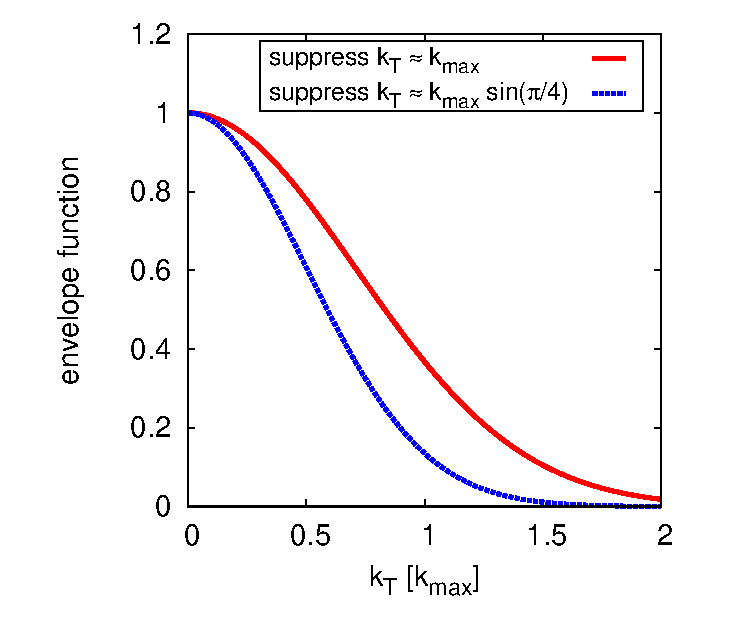
\includegraphics[width=10cm]{envelope}
    \caption{Used envelope functions to suppress $k_T\simeq k_{\rm max}$ (solid) and $k_T\simeq k_{\rm max} \sin(\pi/4)$
     which corresponds to a suppression of emmission angles $\theta \gtrsim \pi/4$. \label{fig:envelope}}
  \end{center}
\end{figure}


%%% Local Variables: 
%%% mode: latex
%%% TeX-master: "manual"
%%% End: 
